%Dokumentinnstillinger:---------------------------------
%Ved å google flitting kan du finne ut hva de forskjellige tingene her betyr, og hvordan du kan gjøre eventuelle endringer.
\documentclass[a4paper,11pt,norsk]{article}
\usepackage[utf8]{inputenc}
\usepackage{a4wide}
\usepackage{lmodern}
\usepackage[T1]{fontenc}
\usepackage{babel}
\setlength{\parindent}{0pt} 
\setlength{\parskip}{2ex}
\usepackage{fixltx2e}
\usepackage{amsmath}
\usepackage[pdftex, pdfborderstyle={/S/U/W 0}]{hyperref}
\usepackage{graphicx}
\usepackage[font=small,labelfont=bf]{caption}
\usepackage{tabularx}
\usepackage{multirow}
\usepackage{float}
\usepackage{subcaption}
\usepackage[RPvoltages]{circuitikz}




\begin{document}

%Headingdel:---------------------------------------------
\begin{minipage}[c]{0.15\textwidth}

\includegraphics[width=2.0cm]{D1/Images/elsys_pos_staaende_ntnu.png}  
\end{minipage}
\begin{minipage}[c]{0.85\textwidth}

\renewcommand{\arraystretch}{1.7}
\large 
\begin{tabularx}{\textwidth}{|X|X|}
\hline
\multicolumn{2}{|l|}{} \\
\multicolumn{2}{|l|}{\huge \textbf{Designnotat}} \\
\multicolumn{2}{|l|}{}  \\
\hline
\multicolumn{2}{|l|}{Tittel: 
%Skriv inn tittel her:------------------------------------------
Oscillator
} \\
\hline
\multicolumn{2}{|l|}{Forfatter: 
%Skriv inn forfattere her:--------------------------------------
Freider Engstrøm Fløan
} \\
\hline
%Skriv inn versjon og dato her her:-----------------------------
Versjon: 2.0 & Dato: 09.05.22
\\
\hline 
\end{tabularx}
\end{minipage}
\normalsize

%Automatisk generert innholdsfortegnelse:------------------

\setlength{\parskip}{0ex}
\renewcommand{\baselinestretch}{0.1}\normalsize
\tableofcontents
\renewcommand{\baselinestretch}{1.00}\normalsize
\setlength{\parskip}{2ex}
\rule{\textwidth}{1pt}
\label{sec:innledning}

\newpage



%Selve rapporten:------------------------------------------
\section{Problembeskrivelse}
\label{sec:problembeskrivelse}

Vi vil undersøke og teste et tilbakekoblet ulineært system, vist i figur \ref{fig:hovedkrets}. Systemet tar ikke inn et inngangssignal, men skal derimot gi ut et sinusformet utgangssignal $y(t)$ med en spesifikk frekvens.

\begin{figure}[H]
  \centering
  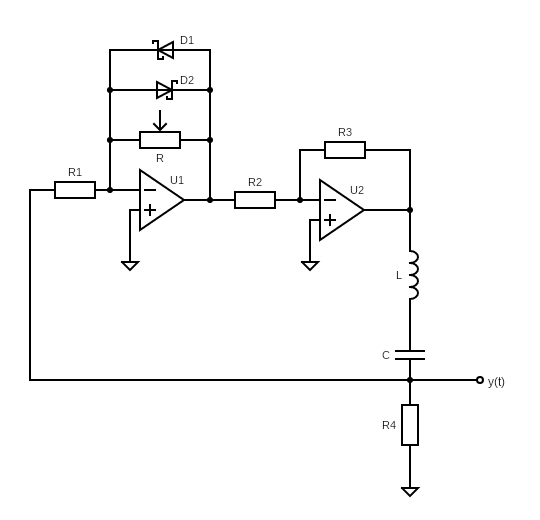
\includegraphics[scale=0.7]{D1/Images/withoutvalues.png}
  \caption{Et ulineært oscillerende system med et RLC-båndpassfilter og en forsterkrets.}
  \label{fig:hovedkrets}
\end{figure}

Det skal undersøkes hvor god frekvensnøyaktighet og hvilke harmoniske forvrengninger som skjer på utgangssignalet $y(t)$. For at denne kretsen skal ha en praktisk nytte trengs det en måte å bestemme hvilken frekvens utgangssignalet gir. Derfor vil vi undersøke om likningen 
\begin{equation}
    f_0 = \frac{1}{2\pi\sqrt{LC}},
    \label{eq:senterfrek}
\end{equation}
som er resonsansfrekvensen til en RLC-krets, er den frekvensen som blir gitt på utgangen $y(t)$. Til slutt skal det undersøkes hvilke verdier for $R$ i figur \ref{fig:hovedkrets} som gir best resultat og hvordan endringer i R gir endringer i fasedigrammet til systemet. 

\section{Metode}
\label{sec:metode}

\subsection{Frekvensnøyaktighet}
\label{sub:frekvensnøyaktighet}
Systemet i figur \ref{fig:hovedkrets} kan deles opp i to deler; et RLC-båndpassfilter og en ulineær forsterker krets. Ved å måle over over $R_4$ vet vi fra~\cite{D2} og~\cite{D3} at likning (\ref{eq:senterfrek}) gir senterfrekvensen til et RLC-båndpassfilter.
Dermed kan likning (\ref{eq:senterfrek}) løses for $C$ og $L$:

\begin{equation}
    C = \frac{1}{L(2\pi f_c)^2}
    \label{eq:kondensatorverdi}
\end{equation}
og
\begin{equation}
    L = \frac{1}{C(2\pi f_c)^2}
\end{equation}
for å finne komponentveridene til båndpassfilteret. 

I en ideel krets ville ikke dette systemet begynt å oscillere, men på grunn av støy som er tilstede i nesten alle praktiske situasjoner begynner systemet gjennom båndpassfilteret å oscillere. Oscillasjonene øker derifra til et punkt der forsterkretsen stabiliserer seg å systemet gir ut resonansfrekvensen til RCL-kretsen~\cite{notat}. For å oppnå høy frekvensnøyaktighet er det nyttig å ha svært nøyaktige komponentverdier som kan oppnås ved måling og utregning. 

Forsterkretsen er koblet opp med to operasjonsforsterker i serie. $U_1$ er koblet opp med et potensiometer og to schottky-dioder i parallell. Hensikten til diodene er å skape ulineæritet slik at frekvenser kan genereres. Egenskapene til schottky-dioder er nyttig i denne kretsen, da de ofte har en lav foroverspenningsfall (150–450 mV), rask reverseringstid (på til av) og er derfor egnet for høye frekvenser~\cite{Schottky}. \newline
Operasjonsforsterkere koblet med inngangssignalet til den negative inngangen og jord til den positive i tillegg til å være tilbakekoblet er en inverterende forsterker, se figur \ref{fig:inv}. Forsterkningen til en slik oppkobling er gitt ved likningen: 

\begin{equation}
    Forsterkning\;[G] = \frac{Utgang}{Inngang} = -\frac{R_2}{R_1}.
    \label{eq:opamp}
\end{equation}

\begin{figure}[H]
  \centering
  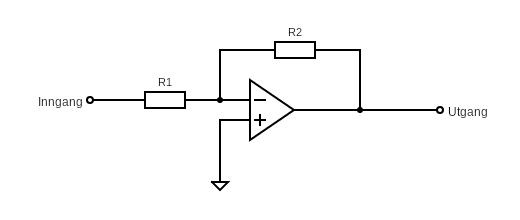
\includegraphics[scale=0.6]{D1/Images/inv.png}
  \caption{Inverterende operasjonsforsterker.}
  \label{fig:inv}
\end{figure}

I figur \ref{fig:hovedkrets} er to slike operasjonsforsterker-kretser koblet i serie, der $U
_2$ gir en forsterkning på $G = -1$ som har som hensikt å snu signalet tilbake til samme fortegn som inngangsignalet til $U_1$. 

\subsection{Overharmonisk forvrengning og grunnfrekvens}
\label{sub:overharmonisk}

Overharmonisk forvrenging er genererte frekvenser som oppstår som et resultat av en ulineær krets. Disse frekvensene er et multiplum av grunnfrekvensen og summen av alle frekvensene gir utgangssignalet $y(t)$~\cite{D3}. Båndpassfilteret til systemet demper frekvensene rundt grunnfrekvensen, men det er vanskelig å få de helt vekk. 

Signal-til-Distorsjonsforhold sier noe om hvor godt resultatet $y(t)$ er i forhold til realisert resultat $\hat{x}_k(t)$, som er summen av $y(t)$ og et distorsjonssingal $d(t)$. Ved bruk av Parsevals sats forklart i ~\cite[Eit kvalitetsmål, s. 3-4)]{notat} er SDR gitt ved et logaritmisk mål 
\begin{equation}
    \text{SDR[dB]} = 10\text{lg}\frac{V^2_{y}}{V^2_{\hat{y}}-V^2_{y}}
    \label{eq:SDR}
\end{equation}
der $V^2_{y}$ er effektveridene (RMS) til $y(t)$ og $V^2_y$ er amplituden til frekvenskomponenten til $y(t)$. SDR $\xrightarrow{}$ $\infty$ når $V^2_{\hat{y}}$ $\xrightarrow{}$ $V^2_{y}$, dermed impliserer en høy SDR et godt resultat. 
\subsection{Endringer i R}
For å undersøke hvordan endringer i R fra fra figur \ref{fig:hovedkrets} kan man se på et fasediagram av systemet. Ved å se på de trigonometriske egenskapene:
\begin{equation}
    \text{sin}'(x) = \text{cos}(x) =  \text{sin}(x + \frac{\pi}{2})
\end{equation}
er en sinusbølge derivert en cosinusbølge eller en 90 graders faseforskjøvet sinusbølge. Utgangssignalet $y(t)$ kan derfor plottes mot spenningen over spolen $L$, fordi spolen $L$ er relativt 90 grader faseforskjøvet. Ved å se på hvor sirkulær fasediagrammet er kan det si noe om hvor godt resultat systemet gir ut. 

\section{Realisering og test}
\label{sec:realisering}
\subsection{Realisering}
Signalet som systemet skal generere er et sinussignal på $5050Hz$.

Realisering av systemet er vist i figur \ref{fig:oppkobling} med skjematisk oppkobling vist i figur \ref{fig:schematic} og komponentverdier i tabell \ref{tab:komp}.

\begin{figure}[H]
  \centering
  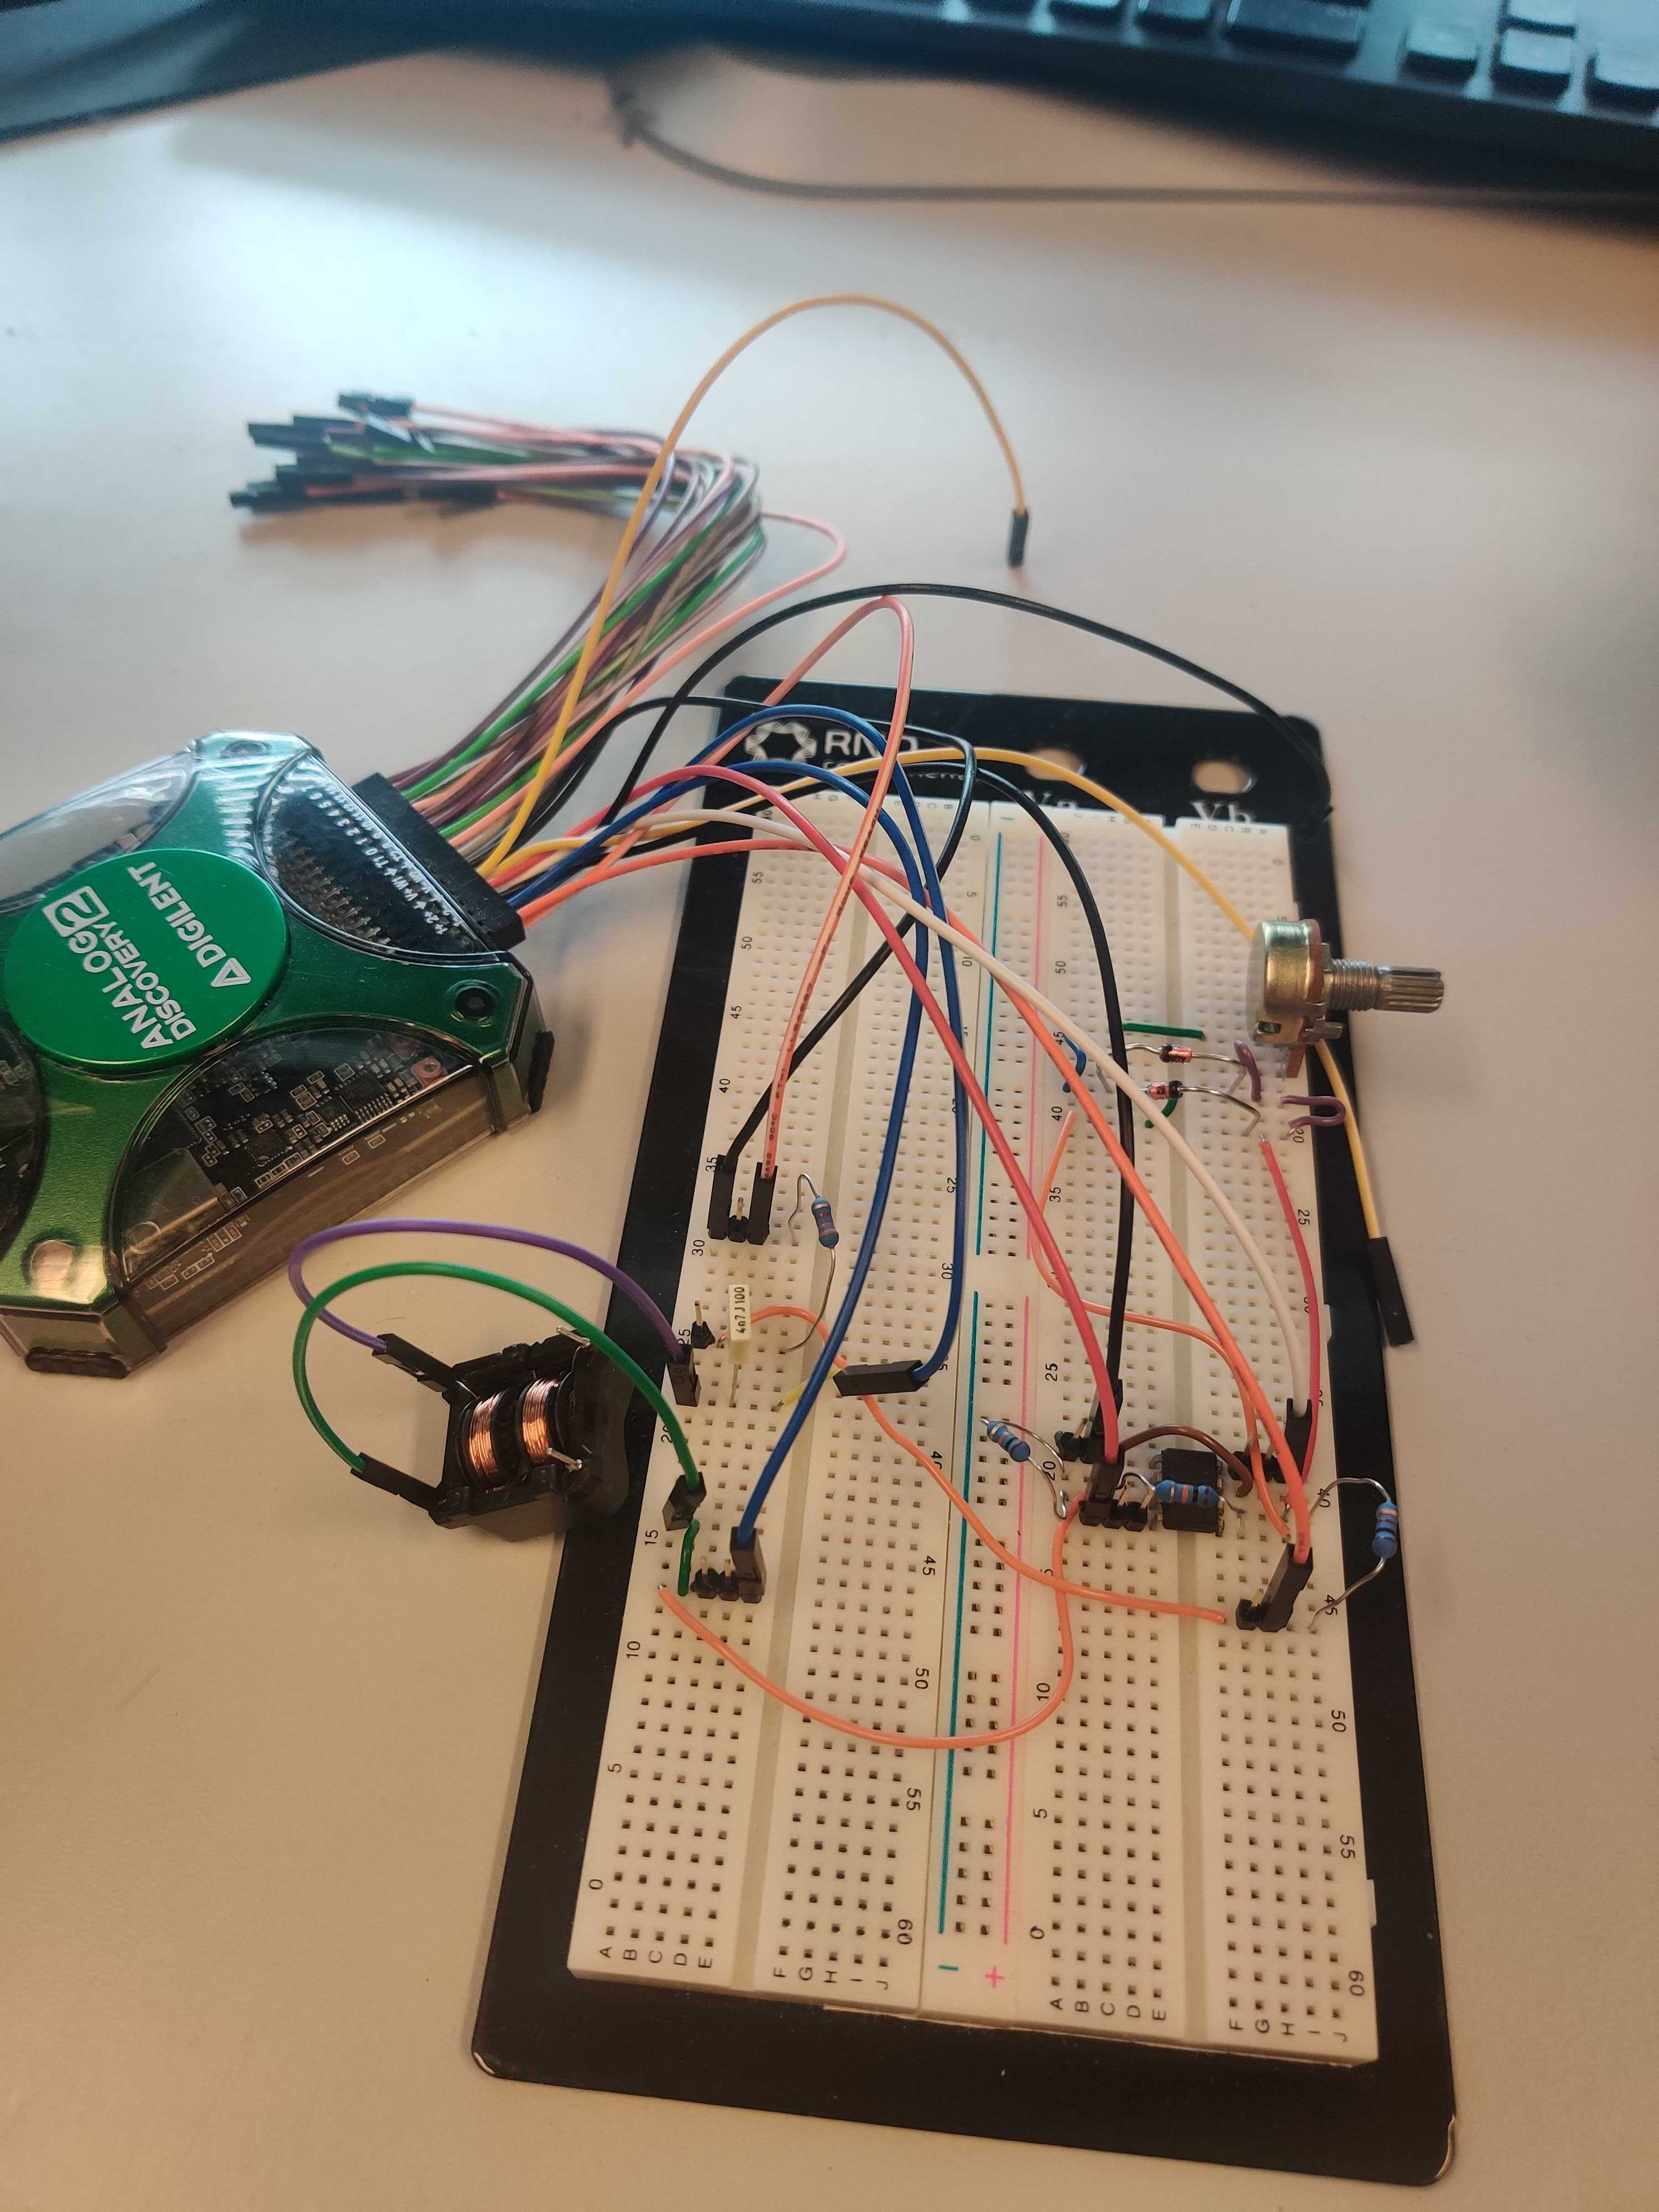
\includegraphics[scale=0.085]{D1/Images/IMG_20220507_153928.jpg}
  \caption{Oppkobling av realisert krets på koblingsbrett.}
  \label{fig:oppkobling}
\end{figure}

\begin{figure}[H]
  \centering
  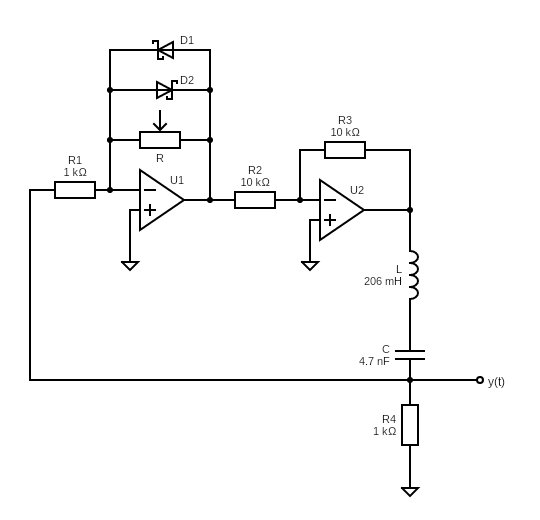
\includegraphics[scale=0.65]{D1/Images/withValues.png}
  \caption{Skjematisk fremstilling av realisert krets.}
  \label{fig:schematic}
\end{figure}

\begin{table}[H]
  \centering
  \caption{Komponenter og deres standardverdier, samt målte verdier.}
  \label{tab:komp}
  \begin{tabular}{|c|c|c|}
    \hline\hline
    Komponenter & Standardverdi & Målt verdi \\
    \hline\hline
    $R$   & $0-10k$ $\Omega$ & $0-9.77$ $\Omega$\\
    \hline
    $R_1$   & $1k$ $\Omega$ & $979$ $\Omega$\\
    \hline
    $R_2$   & $10k$ $\Omega$ & $9.77$ $\Omega$\\
    \hline
    $R_3$   & $10k$ $\Omega$ & $9.67$ $\Omega$\\
    \hline
    $R_4$   & $1k$ $\Omega$ & $980$ $\Omega$\\
    \hline
    $L$   & $100$ mH       & $206$ mH\\
    \hline
    $C$   & $5$ nF       & $4.92$ nF\\
    \hline\hline
    Komponent & Navn produsent &\\
    \hline
    D1 og D2 & Ukjent &\\
    \hline
    U1 og U2 & $LF353P$ &\\
    \hline
  \end{tabular}
\end{table}

Med en tilgjengelig spole $L$ på $206mH$ og ønsket senterfrekvens på filteret til $5050Hz$ kan kondensatorverdien til kretsen regnes ut med likningen (\ref{eq:1}):
\begin{equation}
    \text{C} = \frac{1}{206\text{mH}(2\pi 5050\text{Hz})^2} \approx 4.82 \text{nF}
\end{equation}

Fra likning (\ref{eq:opamp}) ser vi at $R$ må være større enn $R_1$ for å få en forsterkning av inngangssignalet. Derfor er det nyttig med et potensiometer for $R$ som kan justeres til høyere verdi enn $R_1$. 

\subsection{Test}

Figur \ref{fig:faseplott} viser hvordan systemet responderer på endringer av $R$ ved å plotte utgangsignalet $y(t)$ og spenningen over spolen $L$. Figur \ref{fig:faseplott}a viser den laveste verdien for $R$ der systemet fremdeles gir ut et signal. Fra likning (\ref{eq:opamp}) vil $U_1$ ikke forsterke signalet hvis $R \le R_1$, slik at systemet slutter å fungere.
I figur \ref{fig:faseplott}d er potensiometeret $R$ koblet ut slik at det blir en åpen krets eller en tilnærmet uendelig motstand.  
Fra faseplottene i figur \ref{fig:faseplott}, der $y(t)$ er plottet mot $V_L$, gir lavere motstand mindre forvrengning på utgangssignalet. Derimot er det en grense på hvor lav verdi $R$ kan ha. 

\begin{figure}
\centering
    \begin{subfigure}{0.45\linewidth}
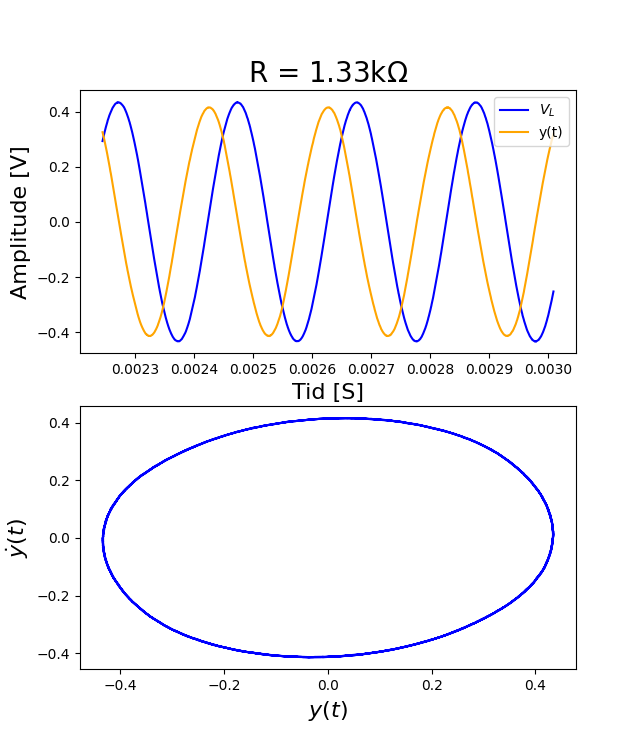
\includegraphics[width=\linewidth]{D1/Images/1.png} 
    \caption{}
\label{fig:1a}
    \end{subfigure}\hfill
    \begin{subfigure}{0.45\linewidth}
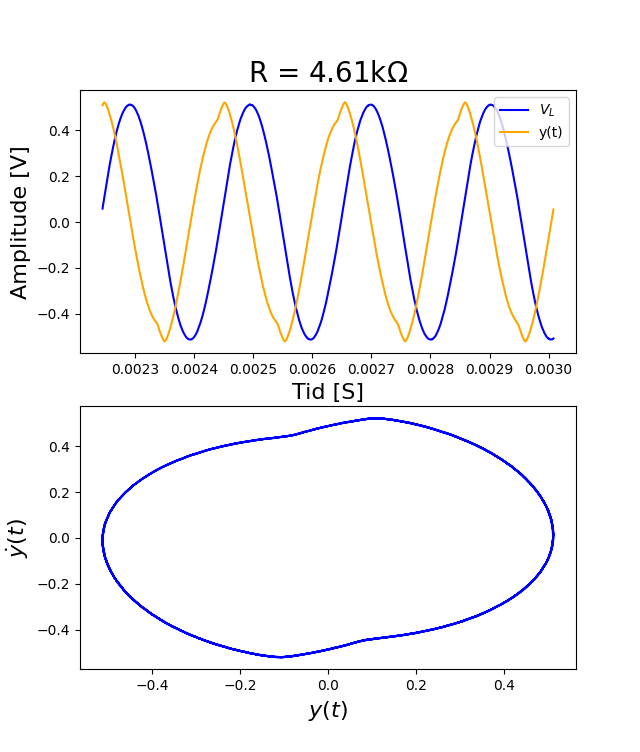
\includegraphics[width=\linewidth]{D1/Images/4.png}
    \caption{}
\label{fig:1a}
    \end{subfigure}
    \begin{subfigure}{0.45\linewidth}
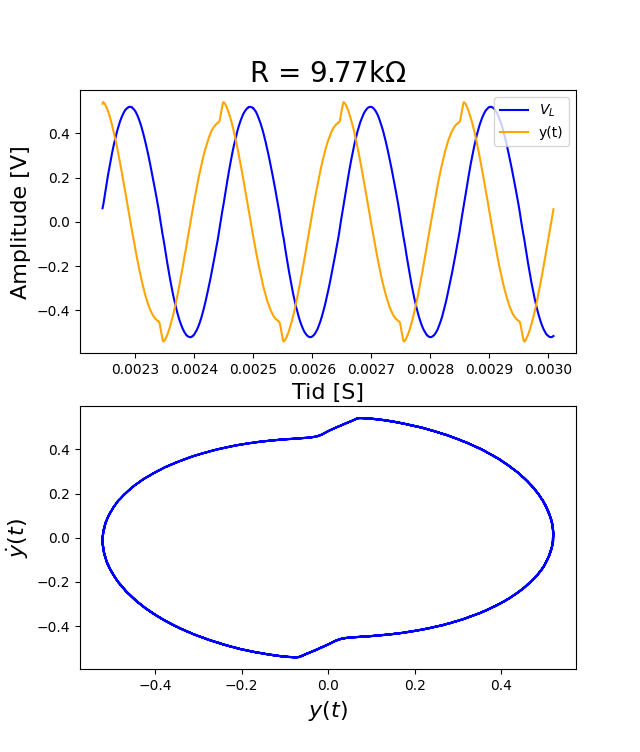
\includegraphics[width=\linewidth]{D1/Images/9.png}
    \caption{}
\label{fig:1a}
    \end{subfigure}\hfill
    \begin{subfigure}{0.45\linewidth}
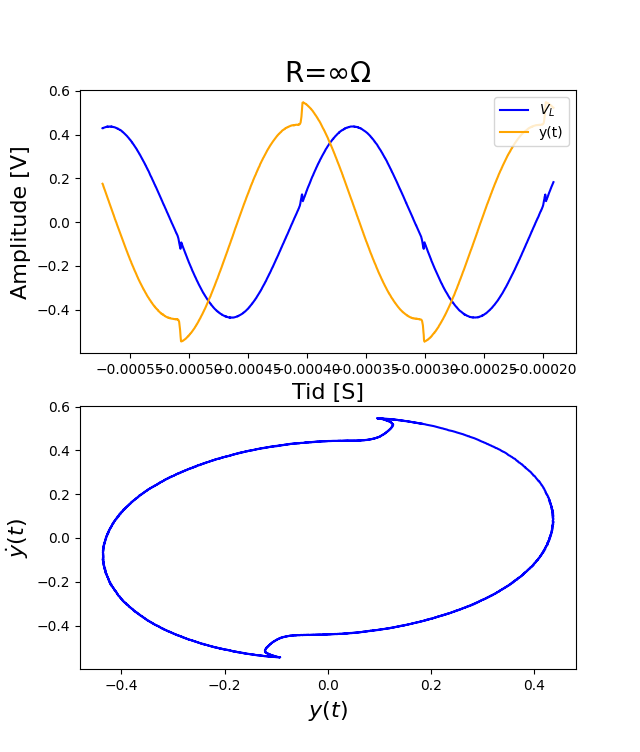
\includegraphics[width=\linewidth]{D1/Images/inf.png}
    \caption{}
\label{fig:1a}
    \end{subfigure}
\caption{Osiloskopsanalyse av forskjellige verdier av $R$.}
    \label{fig:faseplott}
    \end{figure}

\begin{figure}[H]
  \centering
  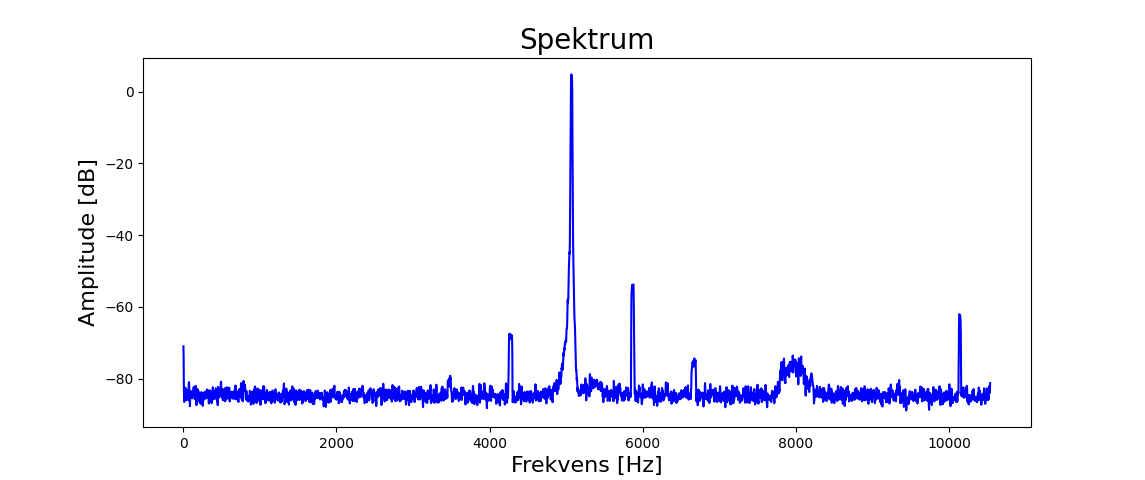
\includegraphics[scale=0.442]{D1/Images/spectrum.png}
  \caption{Spektrumanalyse av $y(t)$ der $R = 1.33k\Omega$.}
  \label{fig:spectrum}
\end{figure}

Ved hjelp av en spektrumanalysator er det mulig å identifisere frekvensene til utgangssignalet $yk(t)$ som vist i figur \ref{fig:spectrum}. Grunnfrekvensen ble målt til $5042$, men det er flere harmoniske komponenter til stedet som skaper noe støy. 

For å analyserer forvregingsgraden på utgangssignalet $y(t)$ for å si noe om kvaliteten på utgangssignalet ved lavest mulig $R$ gir likning (\ref{eq:SDR}):

\begin{equation}
    \text{SDR[dB]} = 10\text{lg}\frac{170.2\text{mV}^2}{171.8\text{mV}^2-170.2\text{mV}^2} \approx 52.9\text{dB}.
    \label{eq:1}
\end{equation}

\section{Konklusjon}
\label{sec:konklusjon}
Systemet som ble beskrevet og implementert i dette notatet var en oscillatorkrets som skulle undersøkes. Det ble undersøkt hvordan endringer av $R$ påvirket systemet ved å se på overharmonisk forvregning, grunnfrekvens og frekvensnøyaktighet, der ønsket frekvens var $5050$Hz.
Etter testing og realisering ble et signal med frekvens på $5042$Hz oppnådd med en SDR målt til 52.9.
For å forbedre dette systemet kunne et smalere båndpassfilter blitt brukt, for å få mindre støy på utgangssignalet. Det kunne blitt realisert med flere filtre i serie eller en annen type med smalere båndbredde. 

\section{Takk}

Takk til Orbit NTNU for å gi meg muligheten til bruk av lokalet og alt nødvendig utstyr, samt hjelp av flere medlemmer. 

Takker også mine medstudenter Mathias Askeland, Mahdan Gazimagamahev og Nikolai Andresen for hjelp til oppkobling, feilsøking og produktiv diskusjon rundt prosjektet.

\phantomsection
\addcontentsline{toc}{section}{Referanser}

\begin{thebibliography}{99}
    \bibitem{notat}
        Lundheim L., 
        \textit{Designprosjekt 4: Oscillator}, 
    	Elsys-2022-LL-1, 
    	NTNU,
    	2022.
    \bibitem{notat2}
        Lundheim L., 
        \textit{Teknisk notat: Frekvensmultiplikator}, 
    	Elsys-2021-LL-1, 
    	NTNU,
    	2021.
    \bibitem{D2}
        Fløan F., 
        \textit{Designprosjekt 2: Støyfjerningsfilter}, 
    	NTNU,
    	2022.
    \bibitem{D3}
        Fløan F., 
        \textit{Designprosjekt 3: Frekvensmultiplikator}, 
    	NTNU,
    	2022.
    \bibitem{Schottky}
        Wikipedia bidragsytere, 
        \textit{Schottky diode}, 
    	2022.
\end{thebibliography}

\end{document}